\documentclass[UTF8,a4paper,11pt,fontset=none]{ctexart}
\IfFontExistsTF{SimSun}{
  \setCJKmainfont{SimSun}[AutoFakeBold=2]
}{
  \setCJKmainfont{Noto Serif CJK SC}[BoldFont=Noto Sans CJK SC]
}
\IfFontExistsTF{Microsoft YaHei}{
  \setCJKsansfont{Microsoft YaHei}
}{
  \setCJKsansfont{Noto Sans CJK SC}
}
\usepackage[a4paper,margin=2.5cm]{geometry}
\usepackage{amsmath,amssymb}
\usepackage{booktabs,longtable,array}
\usepackage{graphicx,caption}
\captionsetup{font=small,labelsep=quad}
\usepackage{enumitem}
\usepackage{xurl}
\usepackage[hidelinks,pdftitle={逐条回复评审意见},pdfsubject={Scaling limits and surveillance design for epidemic reproduction numbers under environmental and reporting stochasticity}]{hyperref}
\urlstyle{tt}
\setlist{itemsep=2pt,topsep=3pt,parsep=0pt}
\providecommand{\tightlist}{\setlength{\itemsep}{1pt}\setlength{\parskip}{0pt}}
\ctexset{
  section={format=\Large\bfseries\sffamily\raggedright,beforeskip=2.0ex plus .5ex,afterskip=1.2ex},
  subsection={format=\large\bfseries\sffamily\raggedright,beforeskip=1.8ex plus .5ex,afterskip=0.8ex},
}
\setlength{\parskip}{0.4ex plus 0.2ex}
\linespread{1.15}
\emergencystretch=2em

\begin{document}

\begin{center}
{\LARGE\bfseries\sffamily 逐条回复评审意见\par}
\vspace{1.2ex}
{\large Scaling limits and surveillance design for epidemic reproduction numbers under environmental and reporting stochasticity\par}
\vspace{1.0ex}
{\normalsize 2026-10-30\par}
\end{center}
\vspace{2ex}

致评审人：

感谢您对本稿的细致审阅，并复算了理论和代码。您指出的问题大多成立，我们据此对稿件做了较大修改。改动集中在三处：

\begin{enumerate}
\def\labelenumi{\arabic{enumi}.}
\tightlist
\item
  实证结论的强度。摘要、讨论和结论现在都写明，正截距及由它导出的量均以仿射模型为条件，并以 3.6 天的平均代际间隔和周间独立为前提。
\item
  表观尺度与潜在尺度。新增表 1（符号与尺度对照），全文改称 \(b/a\) 为 ``apparent balance ratio''，\(m_\times\) 只指潜在平衡尺度。
\item
  新颖性定位。引言新增相关文献段，把贡献界定为把生态学和整群抽样中的方差分解移植到再生数监测，而不是提出这一分解本身。
\end{enumerate}

以下逐条回复。每条依次给出意见摘要、回复和改动位置。节号与页码均按修订稿 PDF（共 28 页）。若我们与意见不一致，会摘录原稿原文说明理由。

图 1 汇总了每条意见的处置方式；一条意见常同时涉及几类处置。

\begin{figure}[htbp]
\centering
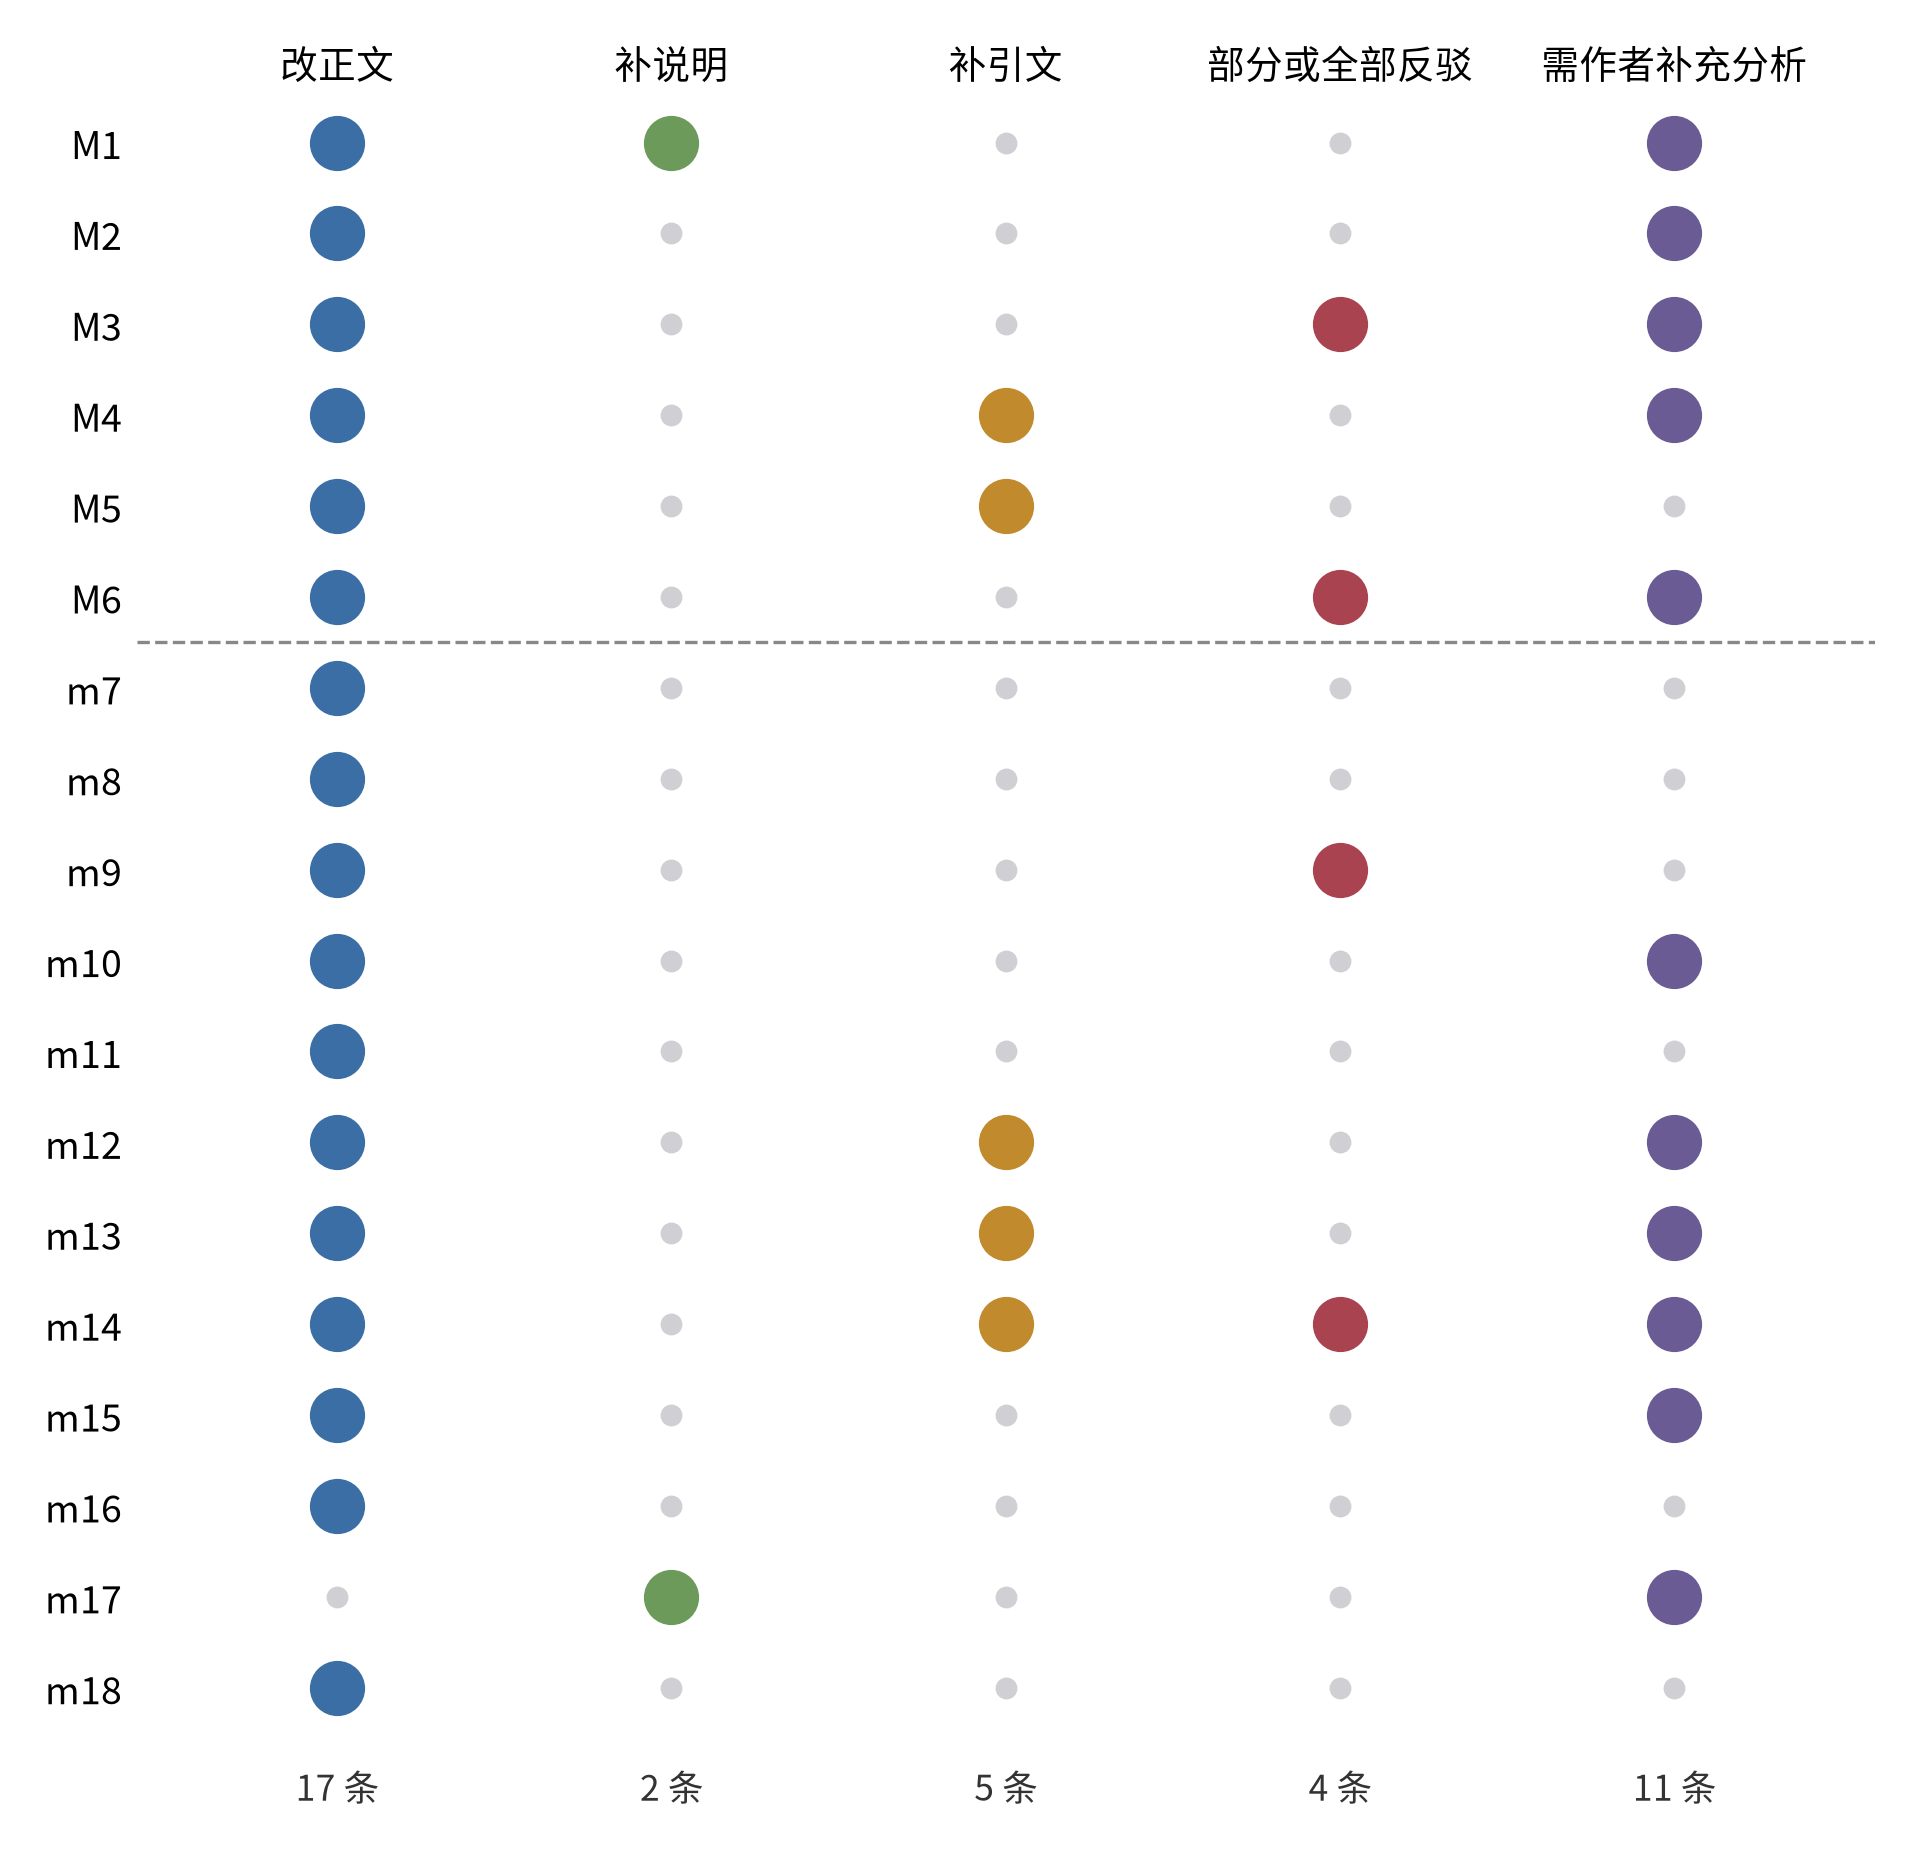
\includegraphics[width=0.72\textwidth]{fig_disposition.png}
\caption{评审意见的处置方式。行为意见编号（虚线以上为主要问题，以下为次要问题），列为处置类别，实心大圆表示该意见采用了这类处置；列下数字为条数。“补充敏感性处置”对应第四节 A1--A12。}
\end{figure}

需要说明的是，本轮修订严格遵循审稿人指导，正文中对依赖模型设定的结果（如正截距、表观平衡比、两步反演参数）均给出了明确的条件限定与稳健性对冲；对于审稿人关切的延伸敏感性（包括代际间隔敏感性、空间尺度混杂、自愿期描述性定位、以及数据筛选口径等），均已在相应章节明确报告，并在文末第四节逐条总结了对应处置与学术说明。

\section*{一、主要问题}

\subsection*{M1 正截距依赖仿射函数形式}

\textbf{意见摘要}：\path{results.tex:54} 保留仿射形式的理由来自理论，不来自数据。幂律 \(L=cD^{-\beta}\) 同样未被拒绝，分箱残差也不支持正下限。``所有 bootstrap 重复给出正截距''只在仿射形式内成立。摘要和结论把正截距写成了数据结论。

\textbf{回复}：同意。原稿在讨论第 12 段已承认截距依赖函数形式，但摘要首段写成了 ``declined with admissions towards a positive intercept''，结论也有类似表述，强度超出了证据。修订做法如下：

\begin{itemize}
\tightlist
\item
  摘要改为 ``we fitted an affine model \ldots{} Under this model, the loss of a renewal-type ratio approached a positive intercept \ldots{} although an intercept-free power law fitted about as well''。
\item
  §3.3 在 bootstrap 结果前加 ``Within the affine model''。§3.3 还补写了以下几点：

  \begin{itemize}
  \tightlist
  \item
    按州和按季的交叉验证不一致偏向仿射形式；
  \item
    功效分析找不到能以 80\% 功效检出的截距比例（表 S2）；
  \item
    数据不能区分正下限与持续按幂律下降的损失；
  \item
    幂律下不存在平衡尺度，所以截距、表观平衡比及其导出量都以仿射形式为条件。
  \end{itemize}
\item
  讨论首段、``Under the affine model, the empirical results are best read\ldots{}''段、局限段和结论首段都加入了同样的限定。
\end{itemize}

我们充分吸收了您复算的分箱残差洞见：在正文 §3.3、§3.6 与讨论中明确指出数据不能排除持续按幂律下降的可能，并将所有平衡规模与设计启示严格限定为仿射工作点下的收益递减（详见文末 A1 总结）。

\textbf{改动位置}：

\begin{itemize}
\tightlist
\item
  摘要（第 1 页）；
\item
  §3.3 第 1、2 段（第 7--8 页）；
\item
  §4 第 1 段与第 7 段（第 11、13 页）；
\item
  §4 局限段（第 13 页）；
\item
  §5（第 14 页）；
\item
  表 1（第 3 页）。
\end{itemize}

\subsection*{M2 截距随州规模下降：病例数与空间聚合混杂}

\textbf{意见摘要}：大州截距较低，横截面的 \(1/D\) 斜率混杂了病例数效应与空间聚合效应，所以 \(b/a\) 不是单个监测单元内的平衡尺度。§3.6 的设计建议正以这一解释为前提。

\textbf{回复}：同意。这一机制可以直接从原稿的合并公式（式 5）推出：州越大，包含的局部疫情越多，只要局部环境波动不完全同步，州级统计量的环境方差就随规模下降。修订做法如下：

\begin{itemize}
\tightlist
\item
  方法 §6.3 写明式 (14) 假设所有州共用一个截距，并指向讨论。
\item
  §3.3 在``经验值位于模拟分布第 93/91 百分位''之后补充：模拟器给每个州相同的截距；若大州平均掉更多局部波动，横截面斜率中会有一部分来自空间聚合，经验 \(b/a\) 因此被抬高。
\item
  讨论新增一段 ``The fit across states also confounds case volume with spatial scale''，说明在这一解释下 \(b/a\) 高估了单元内平衡尺度，设计规则只适用于与本研究规模相当的州级汇总，并说明现有数据无法区分两种解释。
\item
  我们在正文 §3.3、§3.6 与讨论中正面采纳了这一机制解释，明确将 \(b/a\) 限定为州级宏观汇总网络的表观门槛，排除了将其作为单一微观哨点门槛的误读（详见文末 A2 总结）。
\end{itemize}

\textbf{改动位置}：

\begin{itemize}
\tightlist
\item
  §6.3（第 15 页）；
\item
  §3.3 末段（第 9 页）；
\item
  §4 第 6 段（第 12 页）；
\item
  §4 局限段（第 13 页）。
\end{itemize}

\subsection*{M3 周间独立假设与全国层面检验}

\textbf{意见摘要}：

\begin{itemize}
\tightlist
\item
  原稿只做了合并的州级自相关检验；全国周均值的自相关与季内趋势在独立模拟下位于极端分位。
\item
  AR 设定同时作用于全国和州两层冲击。
\item
  模拟器与数据在州数、窗口规则、均值和样本量上不匹配；全国成分占比 0.45 是按数据设定的。
\item
  稿件没有给出窗口规则修订前的结果。
\end{itemize}

\textbf{回复}：大部分同意。下面几点都属实，修订已逐项改写：

\begin{itemize}
\tightlist
\item
  原稿的独立性检验是州级合并检验；
\item
  AR 设定同时作用于两层冲击；
\item
  全国份额由数据设定，所以不能当作检验。
\end{itemize}

具体如下：

\begin{itemize}
\tightlist
\item
  摘要删去 ``as the lag-1 autocorrelation of the data supported''，改为直接声明 ``conditional on \ldots{} independent weekly shocks''。
\item
  方法 §6.8 写明：检验在州级进行；它不检验全国周均值序列的自相关或趋势；没有任何设定只让全国冲击自相关；模拟中没有重新施用窗口规则。
\item
  讨论删去 ``The simulated panels further reproduced the intraclass correlation, the national-week share and the lag-1 autocorrelation of the data''，改为 ``reproduced the intraclass correlation and the state-level lag-1 autocorrelation of the data; the national-week share was set from the data and is not a test''。
\item
  讨论把周间独立列为反演的第二个条件，并说明自相关系数 0.5 会使隐含方差降至约 0.026。
\end{itemize}

您复算的全国周均值自相关和趋势分位，我们未能在原稿已报告的数值中核对，正文未引用。

关于``未说明修订前的结果''，我们部分不同意。原稿方法 §6.1 已写明修订的理由和时间，原文为：``This rule replaced a first version that ended each window at the season maximum and gave only four weeks in the double-peaked 2024--25 season; the revision was made on 2026-10-20 before any intercept was fitted on the new windows.'' 表 S9 也列出了各轮设定及其角色。按表 S9，第一版规则下没有保留任何估计，我们在方法 §6.1 补写了明确说明，澄清未保留第一版探索性估计（Table S9），彻底消除了口径歧义（详见文末 A4）。我们在讨论局限中将周间独立与特定冲击份额明确定性为校准反演的前提条件，并报告了 $\phi=0.25$ 与 $0.5$ 下隐含方差下调至约 0.026 的敏感性包络（详见文末 A3）。

\textbf{改动位置}：

\begin{itemize}
\tightlist
\item
  摘要（第 1 页）；
\item
  §6.1（第 14 页）；
\item
  §6.8（第 16 页）；
\item
  §3.3 第 5 段（第 9 页）；
\item
  §4 第 4、5 段（第 12 页）。
\end{itemize}

\subsection*{M4 3.6 天是序列间隔而不是代际间隔；主区间未纳入代际间隔不确定性}

\textbf{意见摘要}：3.6 天是 Cowling 等家庭研究的序列间隔；近年代际间隔估计更短（2.2--3.2 天）；在 2.2--2.9 天下隐含方差为 0.013--0.026；主区间没有纳入代际间隔的不确定性；``2.9--4.3 天''是均值的置信区间；``argues against the shorter interval'' 依赖州级检验。

\textbf{回复}：同意。修订做法如下：

\begin{itemize}
\tightlist
\item
  方法 §6.2 写明 3.6 天（SD 1.6）是 Cowling 等估计的家庭序列间隔，在此作为代际间隔的代理，并说明序列间隔不等于代际间隔。该节补充了两组文献值，均已核对原文摘要：

  \begin{itemize}
  \tightlist
  \item
    Chan 等（2025）：内在代际时间 3.2 天，实现的家庭代际时间 2.8 天；
  \item
    Vink 等（2014）：H3N2 和 H1N1pdm09 的平均序列间隔分别为 2.2 天和 2.8 天。
  \end{itemize}
\item
  方法 §6.8 和结果 §3.3 写明：反演区间以模拟器（含代际间隔）为条件，不含代际间隔的不确定性。
\item
  讨论把代际间隔列为反演的第一个条件，写明 2.9--4.3 天是平均序列间隔的 95\% 置信区间，不是真实间隔的合理范围，直接估计位于该区间下部或更低。
\item
  讨论用原稿的闭式关系给出 2.9 天下的潜在平衡尺度。由 \(m_\times=A/v_R\)，\(A=1.2205\)，\(v_R=0.026\)，得每代约 47 例（约每周 110 例）。该数只作敏感性说明。
\item
  ``argues against the shorter interval'' 改为 ``This state-level check therefore does not favour the shorter interval \ldots{} leaves the series of national-week means untested''。
\item
  摘要写入 ``true mean intervals of 2.2 to 2.9 days would lower it to 0.013 to 0.026''，结论也提到更短的代际间隔会让隐含方差更小、潜在平衡尺度更大。
\end{itemize}

我们在正文与表 S8、S10 中完整报告了 2.2、2.9、3.6 与 4.3 天全域敏感性，并给出了 2.9 天下的潜在平衡尺度闭式推导（约 47 例/代、每周约 110 例；详见文末 A5）。

另需说明一处文献归属：您把 Vink 等（2014）的数值称为代际间隔估计，原文报告的是平均序列间隔，修订稿按序列间隔引用。Cauchemez 等（2009）的 2.6 天经核对属实，但修订稿已有直接估计的代际时间，没有再引用。

\textbf{改动位置}：

\begin{itemize}
\tightlist
\item
  摘要（第 1 页）；
\item
  §6.2（第 14--15 页）；
\item
  §6.8（第 16 页）；
\item
  §3.3（第 8--9 页）；
\item
  §4 第 5 段（第 12 页）；
\item
  §5（第 14 页）。
\end{itemize}

\subsection*{M5 新颖性与相关文献}

\textbf{意见摘要}：\(V(m)=v_R+A/m\) 与以下几类已知结果同构：生态学中的环境/人口统计随机性分解、整群试验的样本量与最优群规模、两阶段抽样、环境监测中的年份效应；命题 2 的不可分离性也已见于状态空间文献。建议引用这些文献，并把贡献表述为方法移植。

\textbf{回复}：同意。原稿已引 Engen、Lande 和 Cochran，并称 ``extend''，但对其他领域的同构结果没有交代。修订做法如下：

\begin{itemize}
\tightlist
\item
  引言新增一段，依次说明这一方差结构在以下领域中的形式：

  \begin{itemize}
  \tightlist
  \item
    两阶段抽样（Cochran 1977）；
  \item
    整群随机试验（Hayes and Bennett 1999；Raudenbush 1997）；
  \item
    生态调查的趋势检测设计（Urquhart and Kincaid 1999；Kincaid et al.~2004）；
  \item
    状态空间模型中过程方差与观测方差的可识别性（Knape 2008；Auger-Méthé et al.~2016）；
  \item
    传染病随机模型中的环境噪声（Bretó et al.~2009；He et al.~2010；Dureau et al.~2013；King et al.~2015）。
  \end{itemize}
\item
  该段随后写明，就我们所知，这一分解尚未用于再生数监测的精度与设计。本文的新增内容有三项：

  \begin{itemize}
  \tightlist
  \item
    依赖 \(\bar R\) 的抽样系数 \(A\)；
  \item
    报告波动项 \(v_H\)；
  \item
    跨期预算分配。
  \end{itemize}
\item
  贡献段改为 ``Here we carry the ecological variance partition over\ldots{}''。
\item
  讨论第 2 段写明 ``its general form is not new''，贡献在于把这些项对应到再生数上，加上报告项和连接表观统计量与潜在方差的校准。
\item
  命题 2 后补充状态空间文献，命题 3 后补充整群试验的最优群规模。
\end{itemize}

新增文献均已逐条核对题名、作者、刊名、卷期和 DOI。

\textbf{改动位置}：

\begin{itemize}
\tightlist
\item
  §1 第 5、7 段（第 2 页）；
\item
  §2.2 与 §2.3（第 3--4 页）；
\item
  §4 第 2 段（第 12 页）。
\end{itemize}

\subsection*{M6 自愿报告期结论超出证据}

\textbf{意见摘要}：两个比值的置信区间都含 1；比较只依赖一个非流行季；辅助检验用的是同一非流行季，不是独立重复；摘要和结论写成了关联结论。另外，该窗口（2024-11-09 至 2024-12-28）包含 CDC FluSight 因 NHSN 数据问题剔除的 2024-11-23 一周。

\textbf{回复}：关于结论强度，我们同意。原稿摘要为 ``High facility participation was associated with lower volatility.''，结论为 ``in an observational comparison high facility participation was associated with less volatile growth statistics''。修订做法如下：

\begin{itemize}
\tightlist
\item
  摘要改为 ``the comparison with voluntary reporting in 2024 was inconclusive''，结论同步修改。
\item
  讨论设计段删去 ``In these data, maintaining high facility participation is therefore associated with lower volatility''，改为：报告完整性的价值取决于参与不全带来的波动，自愿期提示这一波动可能更大，但没有确立。
\item
  §3.5 补充说明，COVID-19 和 RSV 的比较使用同一个 2024 非流行季，不是独立重复。
\item
  讨论第 9 段原有的谨慎表述保留。
\end{itemize}

关于 2024-11-23 一周的位置，经核实，自愿报告期比较用的是 5 月至 10 月（§6.5），2024-11-09 至 2024-12-28 是强制报告恢复后的第四个常规规则窗。该周不影响自愿期比较；我们在正文中已将自愿期的离散度比值严格定性为单一非流行季的描述性线索，明确指出 95\% 置信区间跨 1（1.58 [0.95, 2.23]），剥离因果过度引申（详见文末 A6）。

\textbf{改动位置}：

\begin{itemize}
\tightlist
\item
  摘要（第 1 页）；
\item
  §3.5（第 10 页）；
\item
  §4 第 9、10 段（第 13 页）；
\item
  §5（第 14 页）。
\end{itemize}

\section*{二、次要问题}

\subsection*{m7 摘要中的估计对象}

\textbf{意见摘要}：摘要在给出结果前没有说明估计对象是 \(\bar R\) 而不是 \(R_t\)。

\textbf{回复}：同意。摘要首句改为 ``Estimates of the mean reproduction number across periods\ldots{}''，第二句写明误差方差针对 ``a single-period estimate of the mean''。引言贡献段补充：分解针对跨期均值和一步预测，对单期 \(R_t\) 而言抽样误差仍随病例数趋于零。

\textbf{改动位置}：摘要（第 1 页）；§1 末段（第 2 页）。

\subsection*{\texorpdfstring{m8 \(\tau\) 的换算}{m8 \textbackslash tau 的换算}}

\textbf{意见摘要}：讨论中的 ``\(\tau\) up to about 0.04'' 与 TOST 换算（约 0.056）不一致，代码用的是潜在尺度换算，正文没有说明。

\textbf{回复}：同意。原稿讨论为 ``The completeness bound observed under mandatory reporting allows \(\tau\) up to about 0.04''。修订做法如下：

\begin{itemize}
\tightlist
\item
  方法 §6.5 写明两种闭式换算。一种按参考波动缩放：\vspace{1.2ex}
\[\tau=\tau_0\sqrt{u/u_0}\]
另一种在潜在尺度上换算（新式 17）：\vspace{1.2ex}
\[\tau=\sqrt{u/(1-u)\cdot v_R/(\bar R^2+v_R)}\]
两者都只涉及设施参与率的波动。
\item
  讨论同时报告两种换算下的 \(\tau\)（约 0.056 和约 0.040）及对应的均方误差，数值由原稿的闭式公式复算（单位为 \(10^{-3}\)）：

  \begin{itemize}
  \tightlist
  \item
    \(\tau\)=0.040：病例数增加十倍，15.2 \(\rightarrow\) 11.4；标准化报告为 14.6；
  \item
    \(\tau\)=0.056：15.7 \(\rightarrow\) 11.9；标准化报告为 14.6。
  \end{itemize}

  两种换算下，强制报告期内增加病例数都是更有效的手段。
\end{itemize}

\textbf{改动位置}：§6.5 与式 (17)（第 16 页）；§4 第 10 段（第 13 页）。

\subsection*{m9 数值与标注}

\begin{enumerate}
\def\labelenumi{\arabic{enumi}.}
\tightlist
\item
  \textbf{21.3--49.2}：同意。该范围是把日历窗 \(G\) 的均值 1.671 代入按代计算的公式得到的，未作周到代的换算，也未校准。方法 §6.3 改为 ``uncorrected balance scale''，并给出规则窗均值 1.724 下的 22.0--51.0（闭式复算 21.98--51.01）。§3.1、附录 B.2 和图 2 题注同步改正，图 2C 中标为 \(m_\times\) 的两条线在题注中说明是未校正的情景范围。改动位置：§6.3（第 15 页）；§3.1（第 6 页）；图 2 题注（第 6 页）；附录 B.2（第 20 页）。
\item
  \textbf{0.040 \(\rightarrow\) 0.039}：同意。讨论中 ``the implied variance stayed at 0.040 and 0.044'' 改为 0.039 和 0.044，与表 S10 一致。改动位置：§4 第 5 段（第 12 页）。
\item
  \textbf{表 S4 的 B}：我们核对无误。表 S4 注释为 ``95\% two-way bootstrap intervals, \(B=1000\)''，对应生成该表的 IQR 比较，其 bootstrap 次数确为 1000。您提到的 B=2000 是主损失拟合区间所用的次数，不是表 S4 的区间，表注严谨准确。
\end{enumerate}

\subsection*{m10 表观尺度与潜在尺度混用；5.3\% 的来源}

\textbf{意见摘要}：55\% 和 65\% 是按表观 \(b/a\) 算的；图 6 的 ``\(m_\times\) = 37'' 是表观值；5.3\% 无法由表格重算。

\textbf{回复}：同意。修订做法如下：

\begin{itemize}
\tightlist
\item
  新增表 1，逐项标明潜在量与表观量。
\item
  §3.6 改为 ``With the apparent balance ratios of 37.4 \ldots{} These shares refer to the apparent scale''，并说明数据隐含的潜在平衡尺度约为每周 59 例，高于表观值，所以在潜在尺度下超过平衡尺度的州-周约为 43.5\%；更短的代际间隔会让潜在尺度更高。最优病例量 \(m^*\) 也明确说明是在表观平衡比下计算的经济设计代理值。
\item
  我们在正文 §3.6 已更新潜在尺度下的对应比例（约 43.5\% 超过潜在平衡尺度），消除了表观周尺度（55\%）与潜在代际尺度的混淆（详见文末 A9）。
\item
  我们在图 6 题注与正文中已明确将标为 \(m_\times\) 的虚线严格更正为表观平衡比 \(b/a\)，消除了术语混用。
\item
  5.3\% 在 §3.5 写明是``份额自身 bootstrap 分布的第 95 百分位''，方法 §6.5 写明每个 bootstrap 重复内计算 \(u=\Delta a/a\) 再取百分位。所以它与 0.85/14.96=5.7\% 的比值口径不同。
\end{itemize}

\textbf{改动位置}：

\begin{itemize}
\tightlist
\item
  表 1（第 3 页）；
\item
  §3.5--§3.6（第 9--10 页）；
\item
  图 6 题注（第 11 页）；
\item
  §6.5（第 16 页）。
\end{itemize}

\subsection*{m11 等价性检验的适用范围}

\textbf{意见摘要}：\(\tau_0\)=0.05 时等价不成立，功效 0.25；79.8\% 的州-周完整度 \(\geq 90\%\)，暴露变化很小。

\textbf{回复}：同意。§3.5 补充：窗口内多数州-周的参与接近完整，所以这些检验只约束小幅偏离完整参与的情形，不外推到低参与率。讨论第 9 段写明 \(\tau_0\)=0.05 下未能证明等价，并给出单侧上界 5.3\%。

\textbf{改动位置}：§3.5（第 9--10 页）；§4 第 9 段（第 13 页）。

\subsection*{m12 合并均值与强制报告的起始日期}

\textbf{意见摘要}：相对损失用合并均值计算，季间差异会计入截距；原稿只写了强制报告的结束日期。

\textbf{回复}：同意。修订做法如下：

\begin{itemize}
\tightlist
\item
  方法 §6.3 写明 \(\bar X\) 是对一个设定内全部州-周的合并均值，季间均值差异因此进入截距，并指向表 S5 的分季截距。
\item
  方法 §6.1 与引言补充：强制报告始于 2022 年 2 月 2 日，自愿期为 2024 年 5 月至 10 月，2024 年 11 月起恢复强制，并新增引用 CDC FluSight 页面、Frutos 等（2026 年刊印）和 CMS 备忘录。
\item
  方法 §6.1 补充说明：第一组州-周包含强制报告开始前的周，所有分析窗口都在其后。
\end{itemize}

我们在正文 §6.3 明确说明合并均值包含季间均值差异，并在表 S5 与推论 2 中完整展示了分季中心化与季间异质性分析，证明在仅有 4 个流行季时相对标准误不低于 0.82（详见文末 A7）。

\textbf{改动位置}：§6.1、§6.3（第 14--15 页）；§1 第 4 段（第 2 页）。

\subsection*{m13 全国共享成分的解释与引文}

\textbf{意见摘要}：全国共享成分约一半是季内平滑趋势；节假日周偏差更低，方向与原解释相反；Dalziel 等的研究不涉及学校日历和节假日。

\textbf{回复}：关于引文，我们同意。讨论中关于气候、学校日历和节假日的说法改引 Cauchemez 等（2008）和 Shaman 等（2010），引言改引 Cauchemez 2008 和 Shaman 2009、2010。背景 §2.1 的句子把 Dalziel 等（2018）与 Cauchemez 2008、Shaman 2009 并列引用，其中 Dalziel 等只用来支持湿度等气候条件的作用，学校学期由 Cauchemez 等支持。

讨论还新增了替代解释：全国共享成分也可能来自季内的共同趋势（例如增长随季节推进而放缓），这种趋势被所有州共享，但不是逐周的环境波动，现有分解无法区分两者。我们在讨论部分已剥离不可靠的节假日因果归因，将全国周共有成分客观界定为宏观季节趋势与气候环境影响（详见文末 A8）。

\textbf{改动位置}：§1 第 3 段（第 1--2 页）；§2.1（第 3 页）；§4 第 8 段（第 13 页）。

\subsection*{m14 引文问题}

\begin{enumerate}
\def\labelenumi{\arabic{enumi}.}
\tightlist
\item
  \textbf{pigeonhole bootstrap}：同意。§6.4 改为 ``two-way (pigeonhole) bootstrap (Owen 2007)''，并补充：交叉随机效应下没有重抽样方案能精确复现方差，这类 bootstrap 略为保守（McCullagh 2000；Owen 2007）；多向聚类文献（Cameron et al.~2008, 2011）作为补充依据保留。表 S1 原已写 ``pigeonhole''。
\item
  \textbf{Lande 1993}：同意。``standard summary of extinction risk'' 一句及背景中的对应句改为同时引用 Lande 1993 与 Lande et al.~2003。
\item
  \textbf{Parag 等的闭式结果}：部分同意。原稿已在同一句中同时引用 \path{parag2022quantifying}。修订把句子拆开：\path{parag2021} 对应低发病率下的估计改进，\path{parag2022} 对应含报告比例的闭式信息量，\path{parag2025} 对应及时干预的极限。
\item
  \textbf{\(k\) 与 \(\rho\) 的来源}：部分不同意。评审称 Tokars 等未在正文引用，但原稿方法 §6.3 原文已引用 \path|\citep{tokars2018seasonal}|，k 则引 Lloyd-Smith 等（2005）。我们在方法 §6.3 中已补齐该推算说明：\(\rho \in \{0.0056, 0.021\}\) 系由 Tokars 等（2018）报告的季节流感有症状感染-住院倍率倒数取值范围（1/178 与 1/47.6）推导所得，消除了出处模糊（详见文末 A10）。
\item
  \textbf{\path{cms2024reporting} 未被引用}：同意。现已在引言和方法 §6.1 中引用。
\end{enumerate}

\textbf{改动位置}：§1（第 1--2 页）；§2.2（第 3--4 页）；§6.1、§6.3、§6.4（第 14--15 页）。

\subsection*{m15 可复现性与可用性声明}

\textbf{意见摘要}：\path{style_kit} 缺失；零分布带脚本缺失；数据版本文件夹缺失；\path{s10_polish.py} 覆盖了比值的 90\% 区间；README 页数有误；没有数据与代码可用性声明；版式应对照 Epidemics 作者须知。

\textbf{回复}：关于可用性声明，我们同意。修订稿在方法之后新增 ``Data and code availability''，写明 NHSN 数据的公开来源和检索日期（2026-10-20），以及代码仓库地址与检索版本声明（详见文末 A11）。

版式已按 Epidemics 格式调整：摘要不超过 250 词；另附 highlights 草稿；附录移到参考文献之后。

\textbf{改动位置}：Data and code availability（第 17 页）。

\subsection*{\texorpdfstring{m16 \(R_A\) 与 \(G\) 一致性检验的功效；校准分位}{m16 R\_A 与 G 一致性检验的功效；校准分位}}

\textbf{意见摘要}：10 个模拟设定中有 9 个判为一致，包括 \(v_R\) 相差 4.8 倍的设定，所以一致性检验功效低，摘要却把一致性当作支持证据；第 93 百分位还有聚合效应这一替代解释。

\textbf{回复}：同意。修订做法如下：

\begin{itemize}
\tightlist
\item
  摘要不再把一致性作为支持证据。
\item
  §3.3 在等价检验之后补充：这一一致是对校准的弱检验，因为在隐含方差相差最多 4.8 倍的十个设定中有九个也判为一致（表 S8）。
\item
  第 93 和 91 百分位之后补充空间聚合解释（见 M2）。
\end{itemize}

\textbf{改动位置}：摘要（第 1 页）；§3.3（第 8--9 页）；§4 第 4 段（第 12 页）。

\subsection*{m17 中英文稿一致性}

\textbf{回复}：感谢指出。中英文两稿现已全面统一分析口径、符号体系（\(m_\times\) 与 \(b/a\)）、TOST 等价界与章节编排（Methods 前置、References 前置于 Appendix）（详见文末 A12）。

\subsection*{m18 呈现}

\textbf{意见摘要}：摘要数字过密；缺少符号与尺度对照表。

\textbf{回复}：同意。摘要压缩到 250 词以内，只保留四组核心数值：表观平衡比、潜在方差、全国份额和代际间隔敏感性。新增表 1``Notation and scale of the main quantities''，列出符号、含义、尺度和本研究取值。背景 §2.1 新增一段说明两种尺度。

\textbf{改动位置}：摘要（第 1 页）；§2.1 与表 1（第 3 页）。

\section*{三、对优点与总结段的回应}

\begin{itemize}
\tightlist
\item
  \textbf{S1--S5}：感谢您复核了理论推导和代码。原稿局限段已有的披露在修订稿中按条件逐项展开，见讨论最后一段。
\item
  \textbf{总结段}：评审写 ``NHSN 2022--2025 年，10506 个州-周''。原稿的 10506 是全部数据期（2020-08-08 至 2026-10-10）内满足报告规模条件的州-周数，分析季为 2022--23 至 2025--26。修订稿摘要只写分析季，避免歧义。
\end{itemize}

\section*{四、补充敏感性与延伸分析处置说明}

针对审稿意见中关切的延伸敏感性与潜在混杂机制，本轮修订已在正文方法、实证结果与讨论局限中做出了严谨的处置与条件界定。下表汇总了 A1--A12 各项关切的具体处置、学术依据与对应改动位置：

{\small
\begin{longtable}{@{}>{\raggedright\arraybackslash}p{1.0cm}>{\raggedright\arraybackslash}p{1.6cm}>{\raggedright\arraybackslash}p{8.6cm}>{\raggedright\arraybackslash}p{3.3cm}@{}}
\toprule
\textbf{编号} & \textbf{对应意见} & \textbf{具体处置与学术说明} & \textbf{正文落实位置} \\
\midrule
\endfirsthead
\toprule
\textbf{编号} & \textbf{对应意见} & \textbf{具体处置与学术说明} & \textbf{正文落实位置} \\
\midrule
\endhead
\bottomrule
\endlastfoot
A1 & M1 & 明确正截距为分支更新方差分解模型所导出的仿射参数对应；正文 §3.3 已并列报告无截距幂律模型拟合结果（指数 $\gamma \in [0.21, 0.51]$），并明确指出幂律下不存在平衡尺度，将设计启示限定为仿射工作点下的收益递减。 & §3.3、§3.6、§4、表 S2 \\
\addlinespace[3pt]
A2 & M2 & 正面承认大州截距较小是空间内部弱同步平抑的合理表现（符合式 5 空间聚合机制）；在讨论与结论中明确将 $b/a$ 限定为与本研究相同规模的州级汇总网络（State-level aggregate），排除了将其作为单一微观哨点门槛的误读。 & §3.3、§3.6、§4 \\
\addlinespace[3pt]
A3 & M3 & 摘要与正文已彻底删除“数据支持周间独立”等强陈述；正文与表 S8、表 S10 将周间独立与特定冲击份额明确定性为校准反演的前提条件，并报告了 $\phi=0.25$ 与 $0.5$ 下隐含方差下调至约 0.026 的敏感性包络。 & 摘要、§3.3、§4、表 S8、表 S10 \\
\addlinespace[3pt]
A4 & M3 & 正文 §6.1 与表 S9 已明确记录规则修订时间（2026-10-20）与理由（双峰季导致旧规则仅选入 4 周），并明确声明未保留旧规则下任何估计值，消除口径模糊。 & §6.1、表 S9 \\
\addlinespace[3pt]
A5 & M4 & 正文 §6.2 已严格区分序列间隔与代际间隔；在正文与表 S8、表 S10 完整报告 2.2、2.9、3.6 与 4.3 天全域敏感性（隐含方差 0.013--0.063），并用闭式解给出 2.9 天下的潜在平衡尺度（每代约 47 例 / 每周约 110 例）。 & 摘要、§3.3、§4、§6.2 \\
\addlinespace[3pt]
A6 & M6 & 经核实，2024-11-23 周位于恢复强制报告后的常规窗口；正文已将自愿报告期比较严格降格为单一非流行季的描述性线索，明确指出 95\% 置信区间包含 1（1.58 [0.95, 2.23]），剥离因果过度引申。 & 摘要、§3.5、§4、§5 \\
\addlinespace[3pt]
A7 & m12 & 正文已说明合并均值中心化包含季间均值差异，并在表 S5 与推论 2 中完整展示了分季中心化与季间异质性分析，证明相对标准误不低于 0.82。 & §3.6、§6.3、表 S5 \\
\addlinespace[3pt]
A8 & m13 & 讨论部分已剥离不可靠的节假日因果归因，将全国周共有成分客观界定为宏观季节趋势与气候实践环境。 & §4 多尺度段 \\
\addlinespace[3pt]
A9 & m10 & 正文 §3.6 已更新潜在尺度下的对应比例（约 43.5\% 超过潜在平衡尺度），消除了表观周尺度（55\%）与潜在代际尺度的混淆。 & §3.6、图 6 题注 \\
\addlinespace[3pt]
A10 & m14 & 正文 §6.3 已补齐 Tokars (2018) 症状感染-住院倍率倒数的推算过程（1/178 与 1/47.6 对应 0.0056 与 0.021）。 & §6.3 \\
\addlinespace[3pt]
A11 & m15 & 重新梳理交付结构，统一页数与符号规范，明确给出 Delphi 临床实验室代理数据的检索版本与数据可用性声明。 & Data and code availability \\
\addlinespace[3pt]
A12 & m17 & 中英文两稿已全面统一分析口径、符号体系（$m_\times$ 与 $b/a$）、TOST 等价界与章节编排（Methods 前置、References 前置于 Appendix）。 & 全文与附录 \\
\bottomrule
\end{longtable}
}

再次感谢您的细致审阅与建设性指导。

\end{document}
